\documentclass[12pt]{article}
\usepackage[dvipsnames]{xcolor} % 更多颜色
\usepackage{graphicx} % Required for inserting images
\usepackage{amsmath}
\usepackage{ulem}
\usepackage{cancel}
\usepackage{amssymb}
\usepackage{enumitem}
\usepackage{pdfpages}
\usepackage{pifont}% http://ctan.org/pkg/pifont
\newcommand{\cmark}{\text{\color{ForestGreen}\ding{51}}}%
\newcommand{\xmark}{\text{\color{red}\ding{55}}}%
\usepackage[UTF8]{ctex}

\usepackage[paper=a4paper]{geometry}
\geometry{headheight=2.6cm,headsep=3mm,footskip=13mm}
\geometry{top=2cm,bottom=2cm,left=2cm,right=2cm}

\usepackage{fancyhdr}
\pagestyle{fancy}
\rhead{{\sf\thepage}}
\lhead{JYCの算法竞赛模板}

\fancyhead[L]{\sf\leftmark} 
\fancyhead[R]{\sf\rightmark}

\setlength{\parindent}{0em}

\usepackage{hyperref}
\hypersetup{
	colorlinks=true,
	linkcolor=blue,
	filecolor=magenta,      
	urlcolor=cyan,
	pdftitle={JYCの算法竞赛模板},
	pdfpagemode=FullScreen,
}

\usepackage{listings}
\lstdefinestyle{lfonts}{
	basicstyle   = \footnotesize\ttfamily,
	stringstyle  = \color{purple},
	keywordstyle = \color{blue!60!black}\bfseries,
	commentstyle = \color{olive},
}
\lstdefinestyle{lnumbers}{
	numbers     = left,
	numberstyle = \tiny,
	numbersep   = 1em,
	firstnumber = 1,
	stepnumber  = 1,
}
\lstdefinestyle{llayout}{
	breaklines       = true,
	breakindent	     = 1.1em,
	tabsize          = 4,
	columns          = flexible,
}
\lstdefinestyle{lgeometry}{
	basewidth        = {0.5em, 0.4em},
	xleftmargin      = 20pt,
	xrightmargin     = 0pt,
	frame            = single,
	framesep         = \fboxsep,
	framexleftmargin = 20pt,
}
\lstdefinestyle{lgeneral}{
	style = lfonts,
	style = lnumbers,
	style = llayout,
	style = lgeometry,
	showstringspaces = false,
}
\lstdefinestyle{C++}{
	language = {C++},
	style    = lgeneral,
}

\newcommand{\subsubsubsection}[1]{\paragraph{#1}\mbox{}\\}
\setcounter{secnumdepth}{4} % how many sectioning levels to assign numbers to
\setcounter{tocdepth}{4} % how many sectioning levels to show in ToC

\begin{document}

\title{\vspace{-2cm}\textbf{\huge{JYCの算法竞赛模板}}}
\author{作者:\href{https://codeforces.com/profile/MegalovaniaJ}{MegalovaniaJ}}
\date{}
\maketitle

\tableofcontents

\newpage

{\centering\section{通用}}

\subsection{缺省源}

\lstinputlisting[style=C++]{../Template/Default Source.cpp}

\newpage

\subsection{Mod-Int-Normal 类}

普普通通的整数取模类(注:进行四则运算时,让 Z 在前)

\lstinputlisting[style=C++]{../Template/Mod-Int-Normal.h}

\newpage

\subsection{超级快 C++ 风格 IO}

\lstinputlisting[style=C++]{"../Template/IO.h"}

\newpage

{\centering\section{数据结构}}

\subsection{并查集}

\lstinputlisting[style=C++]{../Template/Data Structures/Disjoint Set Union.h}

\newpage

\subsection{“边带权”并查集}

\lstinputlisting[style=C++]{../Template/Data Structures/Disjoint Set Union Pro.h}

\newpage

\subsection{ST 表}

\lstinputlisting[style=C++]{../Template/Data Structures/Sparse Table.h}

\newpage

\subsection{树状数组}

\lstinputlisting[style=C++]{../Template/Data Structures/Fenwick Tree.h}

\newpage

\subsection{线段树}

封装的不是很好,具体 $Info$ 的传递还是得自己修改源码,没法直接传个 $class$ 进来

初始化时,传入一个一维 $vector$ $a$ 以及它的长度 $n$,数据存储在下标 $1-n$

\lstinputlisting[style=C++]{../Template/Data Structures/Segement Tree.h}

\newpage

\subsection{主席树}

\subsubsection{可持久化权值线段树}

\lstinputlisting[style=C++]{"../Template/Data Structures/Persistent SGT.h"}

\newpage

\subsubsection{可持久化普通线段树}

以\href{http://codeforces.com/problemset/problem/893/F}{CF893F}为模板题

题目大意:给你一颗有根树,点有权值,$m$ 次询问,每次问你某个点的子树中距离其不超过 $k$ 的点的权值的最小值。(边权均为 1,点权有可能重复,$k$ 值每次询问有可能不同)

做法:$dfs$ 得到 $dfn$ 和 $dep$。按照 $dep$ 构建主席树,每次查询 $[dep[u],dep[u]+k]$ 中 $[dfn[u],dfn[u]+siz[u]-1]$ 的最小值,因为 $dep[u]$ 之前 $[dfn[u],dfn[u]+siz[u]-1]$ 不会被更新,所以直接在 $dep[u]+k$ 这个 $root$ 处查询即可

\lstinputlisting[style=C++]{"../Template/Data Structures/Persistent SGT2.h"}

\newpage

\subsection{可持久 01-Trie}

\lstinputlisting[style=C++]{"../Template/Data Structures/Persistent bitTrie.h"}

\newpage

\subsection{珂朵莉树}

\lstinputlisting[style=C++]{../Template/Data Structures/Old Driver Tree.h}

\newpage

\subsection{01-Trie}

\lstinputlisting[style=C++]{../Template/Data Structures/bitTrie.h}

\newpage

\subsection{树链剖分(重链剖分)(LCA模板)}

可以把树链剖分作为 $LCA$ 的模板来使用,比倍增的写法优秀很多

\lstinputlisting[style=C++]{"../Template/Data Structures/Heavy Light Decomposition 1.h"}

\subsection{长链剖分}

\lstinputlisting[style=C++]{"../Template/Data Structures/Heavy Light Decomposition 2.h"}

\newpage

\subsection{倍增法求 LCA}

\lstinputlisting[style=C++]{../Template/Data Structures/Binary Lifting LCA.h}

\newpage

\subsection{平衡树}

\subsubsection{普通平衡树}

非常朴素的 $fhqTreap$,用 $vector$ 实现了一下动态开点

\lstinputlisting[style=C++]{../Template/Data Structures/fhqTreap.h}

\newpage

\subsubsection{文艺平衡树}

依然坚定的使用无旋 $Treap$

\lstinputlisting[style=C++]{../Template/Data Structures/fhqTreap Wenyi.h}

\newpage

\subsection{线段树分治}

以\href{https://www.luogu.com.cn/problem/P5787}{P5787}为模板题

\lstinputlisting[style=C++]{../Template/Data Structures/SGT-offline.h}

\newpage

\subsection{李超线段树}

\lstinputlisting[style=C++]{../Template/Data Structures/Li-Chao-Tree.h}

\newpage

\subsection{吉司机线段树}

把 Wiki 里的代码改了改

\lstinputlisting[style=C++]{../Template/Data Structures/Ji SGT.h}

\newpage

\subsection{猫树}

\lstinputlisting[style=C++]{../Template/Data Structures/CatSGT.h}

\newpage

\subsection{虚树}

模板题:\href{https://codeforces.com/problemset/problem/613/D}{CF613D},核心代码(二次排序法)如下:

\lstinputlisting[style=C++]{../Template/Data Structures/Auxiliary Tree.h}

\newpage

\subsection{两个 set 维护中位数}

\lstinputlisting[style=C++]{../Template/Data Structures/Median.h}

\newpage

\subsection{mindeque}

\lstinputlisting[style=C++]{../Template/Data Structures/mindeque.h}

\newpage

\subsection{归并树}

\lstinputlisting[style=C++]{../Template/Data Structures/Dividing Tree.h}

\newpage

\subsection{左偏树}

\lstinputlisting[style=C++]{../Template/Data Structures/Leftist Tree.h}

\newpage

{\centering\section{图论}}

\subsection{Tarjan(无向图,割点)}

\lstinputlisting[style=C++]{../Template/Graphs/Tarjan(Undirected, Vertex).h}

\newpage

\subsection{Tarjan(无向图,割边)}

\lstinputlisting[style=C++]{../Template/Graphs/Tarjan(Undirected, Bridge).h}

\newpage

\subsection{Tarjan(有向图)}

\lstinputlisting[style=C++]{../Template/Graphs/Tarjan(Directed).h}

\newpage

\subsection{点分治}

\lstinputlisting[style=C++]{../Template/Graphs/Tree Divide.h}

\newpage

\subsection{Kruskal 重构树}

原图中两个点之间的所有简单路径上\textbf{最大边权的最小值} = \textbf{最小生成树}上两个点之间的简单路径上的最大值 = Kruskal 重构树上两点之间的 LCA 的权值

原图中两个点之间的所有简单路径上\textbf{最小边权的最大值} = \textbf{最大生成树}上两个点之间的简单路径上的最小值 = Kruskal 重构树上两点之间的 LCA 的权值

就是看在限制条件下,应该优先走 \textbf{边权小 or 边权大} 的边,然后选择 最小/大生成树

\lstinputlisting[style=C++]{../Template/Graphs/Kruskal RE Tree.h}

\newpage

\subsection{最大流(Dinic)}

初始化需传入点的个数 $n$(不用传什么 $n+1$ 之类的)

调用 \texttt{"MF::dinic(s,t)"} 来获得 $s$ 到 $t$ 的最大流

\lstinputlisting[style=C++]{../Template/Graphs/Max Flow.h}

\newpage

\subsection{费用流(Dinic)}

\lstinputlisting[style=C++]{../Template/Graphs/Min Cost Max Flow.h}

\newpage

{\centering\section{字符串}}

\subsection{字符串哈希(多重哈希)}

修改 HL(hash\_{}layer) 以决定使用几重哈希

init 时,传入字符数组首地址,字符串长度(以及是否倒着求哈希,0和缺省为正着求,1为倒着求)

注意字符数组内数据的下标是 $1-n$ ,$1-n$ ,$1-n$ !!!

\lstinputlisting[style=C++]{../Template/Strings/String Hash Normal.h}

\newpage

\subsubsection{防 Hack 特供版哈希}

1. 打表程序(生成 \texttt{1e9+x} 的质数)

\lstinputlisting[style=C++]{../Template/Strings/Get Big Primes 1e9+x.cpp}

2. 模板修改 \texttt{MOD} 数组

\begin{lstlisting}[style=C++]
namespace HC{//Hash Const
	const int TABLE_SIZE=500;
	const int table[TABLE_SIZE]={7,9,21,33,87,93,97,/*复制打表程序的输出*/};
	//generate modular
	auto GP=[]()->int{return 10'0000'0000+table[rng()%TABLE_SIZE];};
	const int MOD[2]={GP(),GP()};
}
\end{lstlisting}

\newpage

\subsection{KMP}

约定:字符串下标以 $0$ 为起点

定义函数 $\pi[i]$ 表示 $s[0,i]$ 最长的相等的真前缀与真后缀的长度

\lstinputlisting[style=C++]{../Template/Strings/KMP.h}

\subsection{Z 函数(扩展 KMP)}

约定:字符串下标以 $0$ 为起点

定义函数 $z[i]$ 表示 $s$ 和 $s[i,n-1]$ (即以 $s[i]$ 开头的后缀)的最长公共前缀(LCP)的长度,则 $z$ 被成为 $s$ 的 \textbf{Z函数}。特别的,$z[0]=0$

\lstinputlisting[style=C++]{../Template/Strings/Z_Function.h}

\newpage

\subsection{Trie}

\lstinputlisting[style=C++]{../Template/Strings/Trie.h}

\newpage

\subsection{AC 自动机}

\lstinputlisting[style=C++]{../Template/Strings/Aho-Corasick Automaton.h}

\newpage

\subsection{AC 自动机(简单版)}

\lstinputlisting[style=C++]{../Template/Strings/Aho-Corasick Automaton Easy.h}

\newpage

\subsection{回文树}

by fhy

\lstinputlisting[style=C++]{../Template/Strings/回文树.cpp}

\newpage

\subsection{DFA}

\lstinputlisting[style=C++]{../Template/Strings/FSM.h}

\newpage

{\centering\section{数学}}

\subsection{wjr 的数论}

包含 Lucas 定理,ex-CRT 之类的高级科技

\lstinputlisting[style=C++]{../Template/Math/Number Theory (wjr).h}

\newpage

\subsection{高精度}

\href{https://github.com/Baobaobear/MiniBigInteger/blob/main/bigint_tiny.h}{BigIntTiny Template Link},顺便从大佬的 README 里放个 Features preview,不支持的功能就现写吧。

\begin{table}[!ht]
	\centering
	\begin{tabular}{|l|l|l|l|l|}
		\hline
		operators & BigIntHex & BigIntDec & BigIntMini & BigIntTiny \\ \hline
		constructor Bigint & \cmark & \cmark & \cmark & \cmark \\ \hline
		constructor int & \cmark & \cmark & \cmark & \cmark \\ \hline
		constructor char* & \cmark & \cmark & \xmark & \xmark \\ \hline
		constructor string & \cmark & \cmark & \cmark & \cmark \\ \hline
		=Bigint & \cmark & \cmark & \cmark & \cmark \\ \hline
		=int & \cmark & \cmark & \cmark & \cmark \\ \hline
		=string & \cmark & \cmark & \cmark & \cmark \\ \hline
		=char* & \cmark & \cmark & \cmark & \xmark \\ \hline
		<, ==, >, <=, >=, != Bigint & \cmark & \cmark & \cmark & \cmark \\ \hline
		+, -, *, /, \% int & \xmark & \xmark & \xmark & \cmark \\ \hline
		+=, -=, *=, /=, \%= int & \xmark & \xmark & \xmark & \xmark \\ \hline
		+, -, *, /, \% Bigint & \cmark & \cmark & \cmark & \cmark \\ \hline
		+=, -=, *=, /=, \%= Bigint & \cmark & \cmark & \xmark & \xmark \\ \hline
		Base conversion & \cmark & \cmark & \xmark & \xmark \\ \hline
		Efficiency & $\star$ $\star$ $\star$ $\star$ & $\star$ $\star$ $\star$ & $\star$ $\star$ & $\star$ \\ \hline
	\end{tabular}
\end{table}

\lstinputlisting[style=C++]{../Template/Math/BigIntTiny.h}

\subsection{Barrett Reduction}

在模数是题目输入的参量时使用,平时的取模因为模数带有\texttt{const}前缀,编译器会帮我们优化好

对一个值域在\texttt{(-Mod,Mod)}数取模前,如果不确定其正负性,在\textbf{该式最后} \texttt{"+mod"}

以下代码仅在模数 >2 时成立,并且取模完后数的值域为 \texttt{[0,Mod]},故需要在输出答案前\textbf{特判} ans 是否等于 Mod

\lstinputlisting[style=C++]{../Template/Math/Barrett Reduction.h}

\newpage

\subsection{快速幂 \& 矩阵快速幂}

矩阵乘法中,$f$ 为答案矩阵,是一维长为 $n$ 的 $vector$;$a$ 为转移矩阵,是二维 $n\cdot n$ 的 $vector$

传参数时,直接传入当前的 $f$ 与 $a$ 即可

\lstinputlisting[style=C++]{"../Template/Math/QuickPow and MatrixMultiply.h"}

\newpage

\subsection{\_{}\_{}int128 取平方根}

\lstinputlisting[style=C++]{"../Template/Math/Square-128.h"}

\newpage

\subsection{计算 $a^{1/b}$ 的下取整值}

\lstinputlisting[style=C++]{"../Template/Math/Pow_inv.h"}

\subsection{线性筛欧拉函数}

\lstinputlisting[style=C++]{"../Template/Math/Prime and EulerFunction.h"}

\newpage

\subsection{莫比乌斯反演}

这里顺便筛了约数个数, $d_i$ 表示 $i$ 的约数个数, $num_i$ 表示 $i$ 的最小质因子出现次数

\lstinputlisting[style=C++]{"../Template/Math/Mobius.h"}

\newpage

\subsection{扩展欧几里得}

最终会给出一组满足 $a\cdot x+b\cdot y=g$ 的解

\lstinputlisting[style=C++]{"../Template/Math/Exgcd.h"}

\subsection{分数类}

\lstinputlisting[style=C++]{../Template/Math/Fraction.h}

\newpage

\subsection{Mod-Int 类}

用来处理可能对 0 求逆元的情况

\lstinputlisting[style=C++]{../Template/Math/Mod-Int.h}

\newpage

\subsection{异或线性基-普通}

\lstinputlisting[style=C++]{../Template/Math/Linear Basis.h}

\newpage

\subsection{异或线性基-前后缀}

\lstinputlisting[style=C++]{../Template/Math/Linear Basis Suffix.h}

\newpage

\subsection{异或线性基-高斯消元}

\lstinputlisting[style=C++]{../Template/Math/Linear Basis Gaussian.h}

\newpage

\subsection{异或方程组高斯消元}

\lstinputlisting[style=C++]{../Template/Math/Gauss Elimination.h}

\newpage

\subsection{Pollard-Rho 分解质因数}

\lstinputlisting[style=C++]{../Template/Math/Pollard-Rho.h}

\newpage

\subsection{万能欧几里得算法}

\lstinputlisting[style=C++]{../Template/Math/universal-gcd.cpp}

\newpage

\subsection{FFT}

\lstinputlisting[style=C++]{../Template/Math/FFT.h}

\newpage

\subsection{NTT}

\lstinputlisting[style=C++]{../Template/Math/NTT.h}

\newpage


\subsection{Min\_25 筛(超级无敌阉割版)}

by fhy,只能求质数的前缀和

\lstinputlisting[style=C++]{../Template/Math/Min_25.h}

\newpage

\subsection{Schreier Sims}

\lstinputlisting[style=C++]{../Template/Math/Schreier-Sims.h}

\newpage

\subsection{组合数学}

\subsubsection{阶乘相关初始化}

适用于模数为质数,逆元存在的情况

\lstinputlisting[style=C++]{"../Template/Math/Factorial.h"}

\newpage

\subsubsection{组合数相关初始化}

适用于模数随机,逆元不一定存在的情况(搭配 Barrett Reduction 一起使用)

\lstinputlisting[style=C++]{"../Template/Math/Combination.h"}

\newpage

\subsubsection{错位排列}

1. 递推公式(两种任选即可)

$$
\begin{aligned}
	D_{n}&=(n-1)\cdot(D_{n-1}+D_{n-2})\\
	D_{n}&=n\cdot D_{n-1}+(-1)^{n}
\end{aligned}
$$

其中$D$ 的前几项是 $D_1=0, D_2=1, D_3=9, D_4=44, D_5=265 $(\href{http://oeis.org/A000166}{OEIS A000166})

2. 其他关系

错位排列数有一个向下取整的简单表达式,增长速度与阶乘仅相差常数:

$$
D_n=\left\lfloor\frac{n!}{e}\right\rfloor
$$

随着元素数量的增加,形成错位排列的概率 P 接近:

$$
P=\lim_{n\to\infty}\frac{D_n}{n!}=\frac{1}{e}
$$

\subsubsection{卡特兰数}

$H_n=$ 进栈序列为 $1,2,3,\cdots,n$ 的栈的出栈序列个数,以下是一些常见公式

$$
\begin{aligned}
	H_{n}&=\frac{\binom{2n}{n}}{n+1}(n\ge2,n\in\mathbb{N}_{+})\\
	H_{n}&=
	\begin{cases}
		\sum_{i=1}^{n}H_{i-1}H_{n-i} & n\ge2,n\in\mathbb{N}_{+}\\
		1 & n=0,1
	\end{cases}\\
	H_{n}&=\frac{H_{n-1}(4n-2)}{n+1}\\
	H_{n}&=\binom{2n}{n}-\binom{2n}{n-1}
\end{aligned}
$$

\newpage

\subsubsection{斯特林数}

\subsubsubsection{第二类斯特林数}

$n\brace k$,$S(n,k)$,表示将 $n$ 个两两不同的元素,划分为 $k$ 个互不区分的非空子集的方案数

1. 递推公式

$$
{n\brace m}={n-1\brace k-1}+k{n-1\brace k}
$$

边界是 ${n\brace 0}=[n=0]$

2. 通项公式

$$
{n\brace m}=\sum_{i=0}^{m}\frac{(-1)^{m-i}\cdot i^n}{i!\cdot(m-i)!}
$$

待补充:同一行/列的第二类斯特林数的计算

\subsubsubsection{第一类斯特林数}

$n\brack k$,$s(n,k)$,表示将 $n$ 个两两不同的元素,划分为 $k$ 个互不区分的非空轮换的方案数

一个轮换即一个首尾相接的环形排列,如 $[A,B,C,D]=[B,C,D,A]=[C,D,A,B]=[D,A,B,C]$ ,即两个可以通过旋转而相互得到的轮换是等价的。但是,翻转不算旋转,如 $[A,B,C,D]\ne[D,C,B,A]$

1. 递推公式

$$
{n\brack m}={n-1\brack k-1}+(n-1){n-1\brack k}
$$

边界是 ${n\brack 0}=[n=0]$

2. 通项公式

\centerline{没有}

待补充:同一行/列的第一类斯特林数的计算

\newpage

{\centering\section{计算几何}}

\subsection{计算几何基础}

\subsubsection{知识点} % TODO: 修改格式

摘自繁凡的博客和 $yxc$ 的讲义

\textbf{1. 前置知识点}

\textbf{1.1} $\pi=\arccos(-1)$
	
\textbf{1.2} 余弦定理 $c^2=a^2+b^2-2ab\cos\theta$

\textbf{2. 浮点数的比较}

\begin{lstlisting}[style=C++]
const double eps=1e-8; //精度,可按需要增加至1e-12之类的
int sign(double x){ //符号函数
	if(fabs(x)<eps) return 0;
	if(x<0) return -1;
	return 1;
}
int cmp(double x,double y){ //比较函数
	if(fabs(x-y)<eps) return 0;
	if(x<y) return -1;
	return 1;
}
\end{lstlisting}


\textbf{3. 向量}

\textbf{3.1} 点与向量的保存,以及运算符重载

\begin{lstlisting}[style=C++]
using PDD=pair<double,double>;
#define x first
#define y second

PDD operator +(PDD a,PDD b){return PDD{a.x+b.x,a.y+b.y};}
PDD operator -(PDD a,PDD b){return PDD{a.x-b.x,a.y-b.y};}
PDD operator *(PDD a,double k){return PDD{k*a.x,k*a.y};}
PDD operator *(double k,PDD a){return PDD{k*a.x,k*a.y};}
\end{lstlisting}

\textbf{3.2} 内积(点积)$A\cdot B = |A||B|cos\theta$

\textbf{3.2.1} 几何意义:向量 $A$ 在向量 $B$ 上的投影与 $B$ 的长度的乘积
		
\textbf{3.2.2} 代码实现

\begin{lstlisting}[style=C++]
double dot(PDD a,PDD b){
	return a.x*b.x+a.y*b.y;
}
\end{lstlisting}

\textbf{3.3} 外积(叉积)$A\times B=|A||B|\sin\theta$

\textbf{3.3.1} 几何意义:向量 $A$ 与 $B$ 张成的平行四边形的有向面积。$B$ 在 $A$ 的逆时针方向为正
		
\textbf{3.3.2} 代码实现

\begin{lstlisting}[style=C++]
double cross(PDD a,PDD b){
	return a.x*b.y-b.x*a.y;
}
\end{lstlisting}

\textbf{3.4} 常用函数

\textbf{3.4.1} 取模

\begin{lstlisting}[style=C++]
double get_length(PDD a){
	return sqrt(dot(a,a));
}
\end{lstlisting}

\textbf{3.4.2} 计算向量夹角

\begin{lstlisting}[style=C++]
double get_angle(PDD a,PDD b){
	return acos(dot(a,b)/get_length(a)/get_length(b));
}
\end{lstlisting}

\textbf{3.4.3} 计算两个向量构成的平行四边形有向面积

\begin{lstlisting}[style=C++]
double area(PDD a,PDD b,PDD c){
	return cross(b-a,c-a);
}
\end{lstlisting}

\textbf{3.4.4} 向量 $A$ \textbf{顺时针}旋转 $angle$(弧度制)的角度:

\begin{lstlisting}[style=C++]
PDD rotate(PDD a,double angle){
	return PDD{ a.x*cos(angle) + a.y*sin(angle),
		-a.x*sin(angle) + a.y*cos(angle) };
}
\end{lstlisting}

\textbf{4. 点与线}

\textbf{4.1} 直线定理

\textbf{4.1.1} 一般式 $ax+by+c=0$

\textbf{4.1.2} 点向式 $p_0+vt$

\textbf{4.1.3} 斜截式 $y=kx+b$

\textbf{4.2} 常用操作

\textbf{4.2.1} 判断点在直线上 $A\times B=0$

\textbf{4.2.2} 两直线相交(取直线 $p+vt,\space q+wt$ 的交点)

\begin{lstlisting}[style=C++]
//cross(v,w)==0 则两直线平行或者重合,注意特判,这里没加
PDD get_line_inter(PDD p, PDD v, PDD q, PDD w){
	PDD u = p - q;
	double t = cross(w, u) / cross(v, w);
	return p + v * t;
}
\end{lstlisting}

\textbf{4.2.3} 点到直线的距离

\begin{lstlisting}[style=C++]
//点p; 直线由a, b两点表示
double dis2line(PDD p, PDD a, PDD b){
	PDD v1 = b - a, v2 = p - a;
	return fabs(cross(v1, v2) / get_length(v1));
}
\end{lstlisting}

\textbf{4.2.4} 点到线段的距离

\begin{lstlisting}[style=C++]
double dis2seg(PDD p, PDD a, PDD b){
	if (a == b) return get_length(p - a);
	PDD v1 = b - a, v2 = p - a, v3 = p - b;
	if (sign(dot(v1, v2)) < 0) return get_length(v2);
	if (sign(dot(v1, v3)) > 0) return get_length(v3);
	return dis2line(p, a, b);
}
\end{lstlisting}

\textbf{4.2.5} 点在直线上的投影

\begin{lstlisting}[style=C++]
PDD get_line_proj(PDD p, PDD a, PDD b){
	PDD v = b - a;
	return a + v * (dot(v, p - a) / dot(v, v));
}
\end{lstlisting}

\textbf{4.2.6} 点是否在线段上

\begin{lstlisting}[style=C++]
bool on_seg(PDD p, PDD a, PDD b){
	return sign(cross(p - a, p - b)) == 0 && sign(dot(p - a, p - b)) <= 0;
}
\end{lstlisting}

\textbf{4.2.7} 判断两线段是否相交

\begin{lstlisting}[style=C++]
bool seg_inter(PDD a1, PDD a2, PDD b1, PDD b2){
	double c1 = cross(a2-a1, b1-a1), c2 = cross(a2-a1, b2-a1);
	double c3 = cross(b2-b1, a1-b1), c4 = cross(b2-b1, a2-b1);
	// 有if则允许线段在端点处相交,无if则不允许,根据需要添加
	if(!sign(c1) && !sign(c2) && !sign(c3) && !sign(c4)){
		bool f1 = on_seg(b1, a1, a2);
		bool f2 = on_seg(b2, a1, a2);
		bool f3 = on_seg(a1, b1, b2);
		bool f4 = on_seg(a2, b1, b2);
		bool f = (f1|f2|f3|f4);
		return f;
	}
	return (sign(c1)*sign(c2) < 0 && sign(c3)*sign(c4) < 0);
}
\end{lstlisting}

\textbf{5. 多边形}

\textbf{5.1} 三角形

\textbf{5.1.1} 面积

\textbf{5.1.1.1} 叉积

\textbf{5.1.1.2} 海伦公式
$$
\begin{aligned}
	p &= \frac{a + b + c}{2}\\
	S &= \sqrt{p(p - a)\cdot(p - b)\cdot(p - c)}
\end{aligned}
$$

\textbf{5.1.2} 三角形四心

\textbf{5.1.2.1} 外心,外接圆圆心

三边中垂线交点。到三角形三个顶点的距离相等

\textbf{5.1.2.2}内心,内切圆圆心

角平分线交点,到三边距离相等

\textbf{5.1.2.3} 垂心

三条垂线交点

\textbf{5.1.2.4} 重心

三条中线交点

到三角形三顶点距离的平方和最小的点

三角形内到三边距离之积最大的点

\textbf{5.2} 普通多边形,通常按逆时针存储所有点

\textbf{5.2.1} 定义

\textbf{5.2.1.1} 多边形
由在同一平面且不再同一直线上的多条线段首尾顺次连接且不相交所组成的图形叫多边形

\textbf{5.2.2.2} 简单多边形
简单多边形是除相邻边外其它边不相交的多边形

\textbf{5.2.2.3} 凸多边形
过多边形的任意一边做一条直线,如果其他各个顶点都在这条直线的同侧,则把这个多边形叫做凸多边形
任意凸多边形外角和均为 $360^{\circ}$
任意凸多边形内角和为 $(n−2)180^{\circ}$

\textbf{5.2.2} 常用函数

\textbf{5.2.2.1} 求多边形面积(不一定是凸多边形)
我们可以从第一个顶点出发把凸多边形分成n − 2个三角形,然后把面积加起来。

\begin{lstlisting}[style=C++]
double polygon_area(vector<PDD>p){
	double s = 0;
	for (int i = 1; i + 1 < p.size(); i ++ )
	s += cross(p[i] - p[0], p[i + 1] - p[i]);
	return s / 2;
}
\end{lstlisting}

\textbf{5.2.2.2} 判断点是否在多边形内(不一定是凸多边形)
      
a. 射线法,从该点任意做一条和所有边都不平行的射线。交点个数为偶数,则在多边形外,为奇数,则在多边形内

b. 转角法

\textbf{5.2.2.3} 判断点是否在凸多边形内

只需判断点是否在所有边的左边(逆时针存储多边形)

\textbf{5.2.2.4} 皮克定理

皮克定理是指一个计算点阵中,顶点在格点上的多边形面积的公式:

$$
S = a + \frac{b}{2} - 1
$$

其中 $a$ 表示多边形内部的点数,$b$ 表示多边形边界上的点数,$S$ 表示多边形的面积。

\textbf{6. 圆}

\textbf{6.1} 圆与直线交点

\textbf{6.2} 两圆交点

\textbf{6.3} 点到圆的切线

\textbf{6.4} 两圆公切线

\textbf{6.5} 两圆相交面积

\newpage

\subsubsection{完整代码}

\lstinputlisting[style=C++]{"../Template/Geometry/Basic.h"}

\newpage

\subsection{凸包}

\subsubsection{代码 1(动态凸包)(by fhy)}

\lstinputlisting[style=C++]{"../Template/Geometry/动态凸包.cpp"}

\newpage

\subsubsection{代码 2(动态凸包 + 全是整点)(by fhy)}

\lstinputlisting[style=C++]{"../Template/Geometry/整点の凸包.cpp"}

\newpage

\subsubsection{代码 3(普通凸包)(by jyc)}

\lstinputlisting[style=C++]{"../Template/Geometry/Andrew.h"}

\newpage

\subsection{闵可夫斯基和}

\lstinputlisting[style=C++]{"../Template/Geometry/Minkowski.h"}

\subsection{点到凸包距离}

如果点在凸包内, 距离就是 0

\lstinputlisting[style=C++]{"../Template/Geometry/DisPointPoly.h"}

\newpage

\subsection{半平面交}

by fhy

\lstinputlisting[style=C++]{"../Template/Geometry/半平面交.cpp"}

{\centering\section{杂项}}
\subsection{竞赛向配置vscode}

\begin{center}
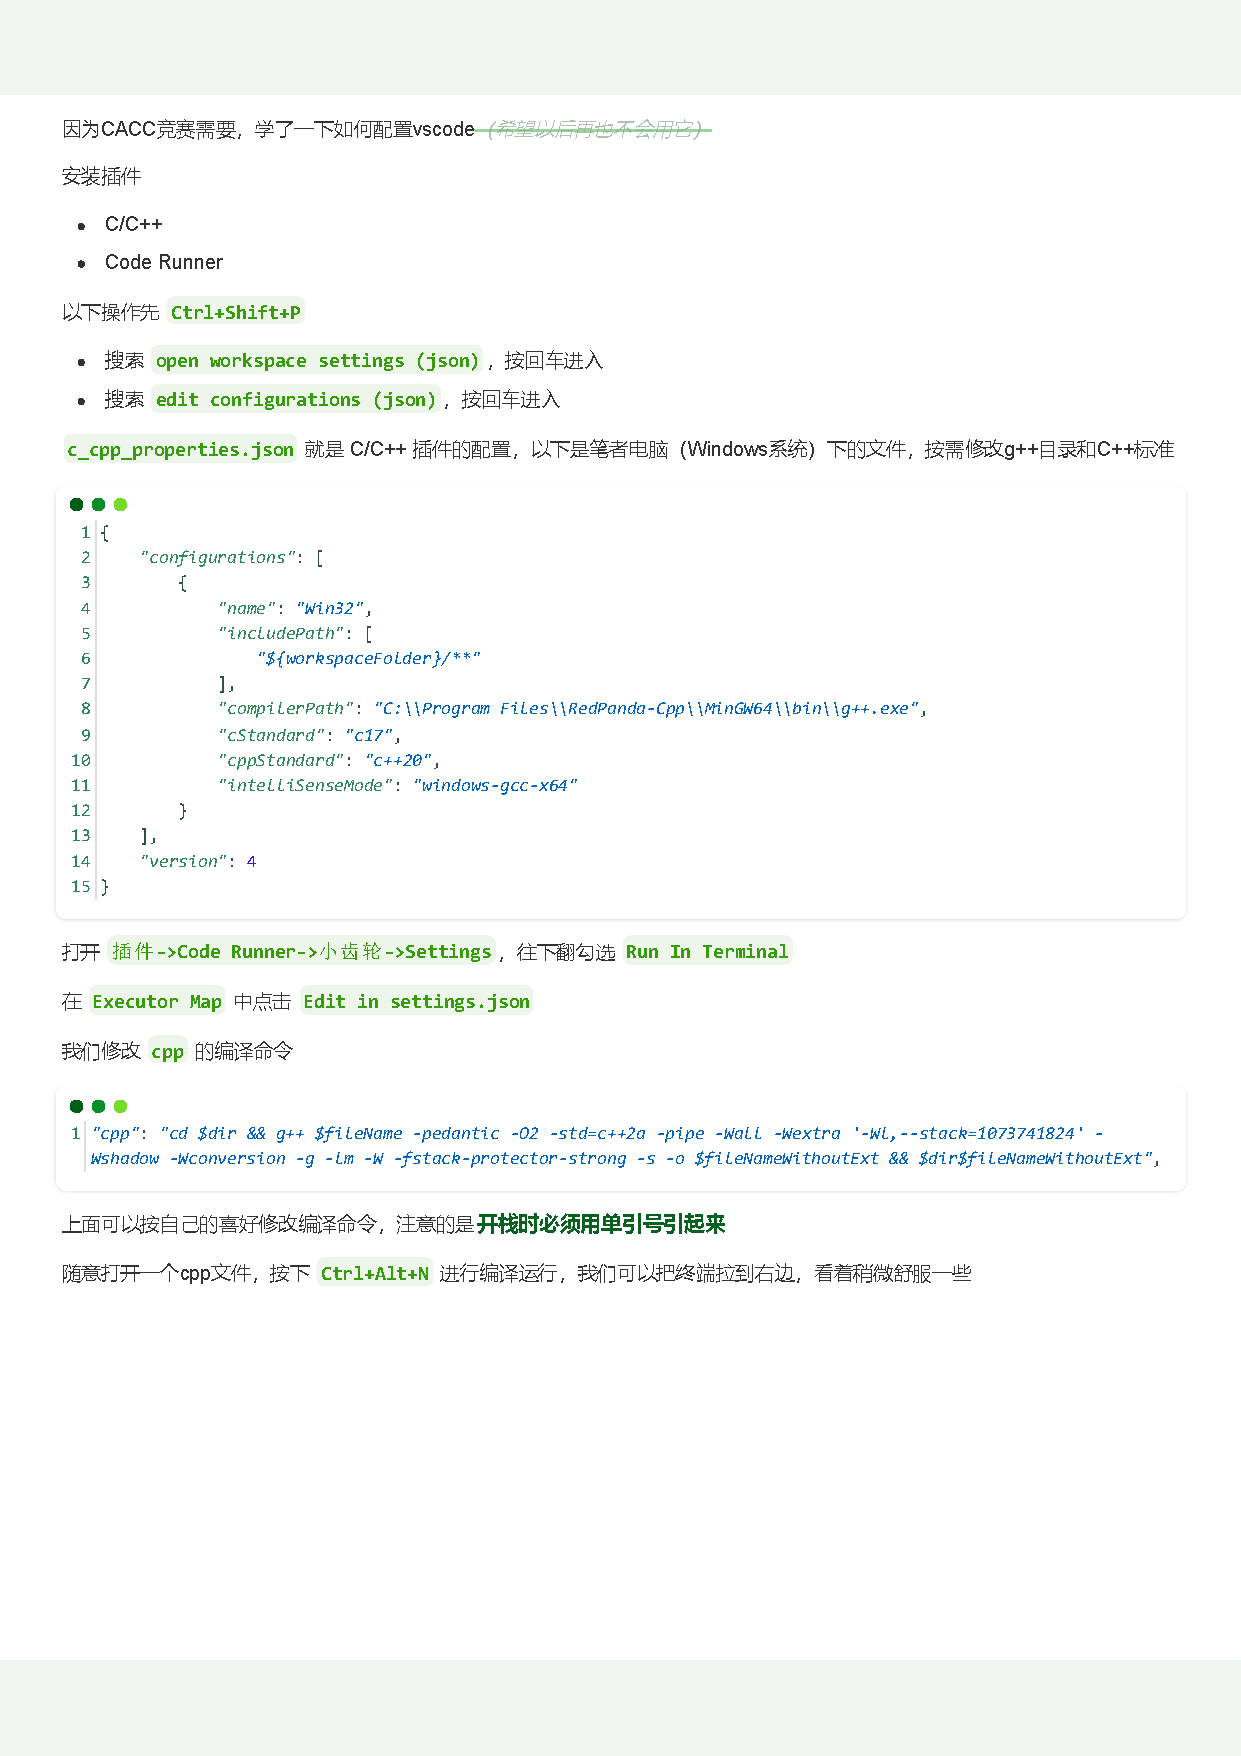
\includegraphics[width=1.1\textwidth]{"../Template/Other/vscode.pdf"}
\end{center}
% 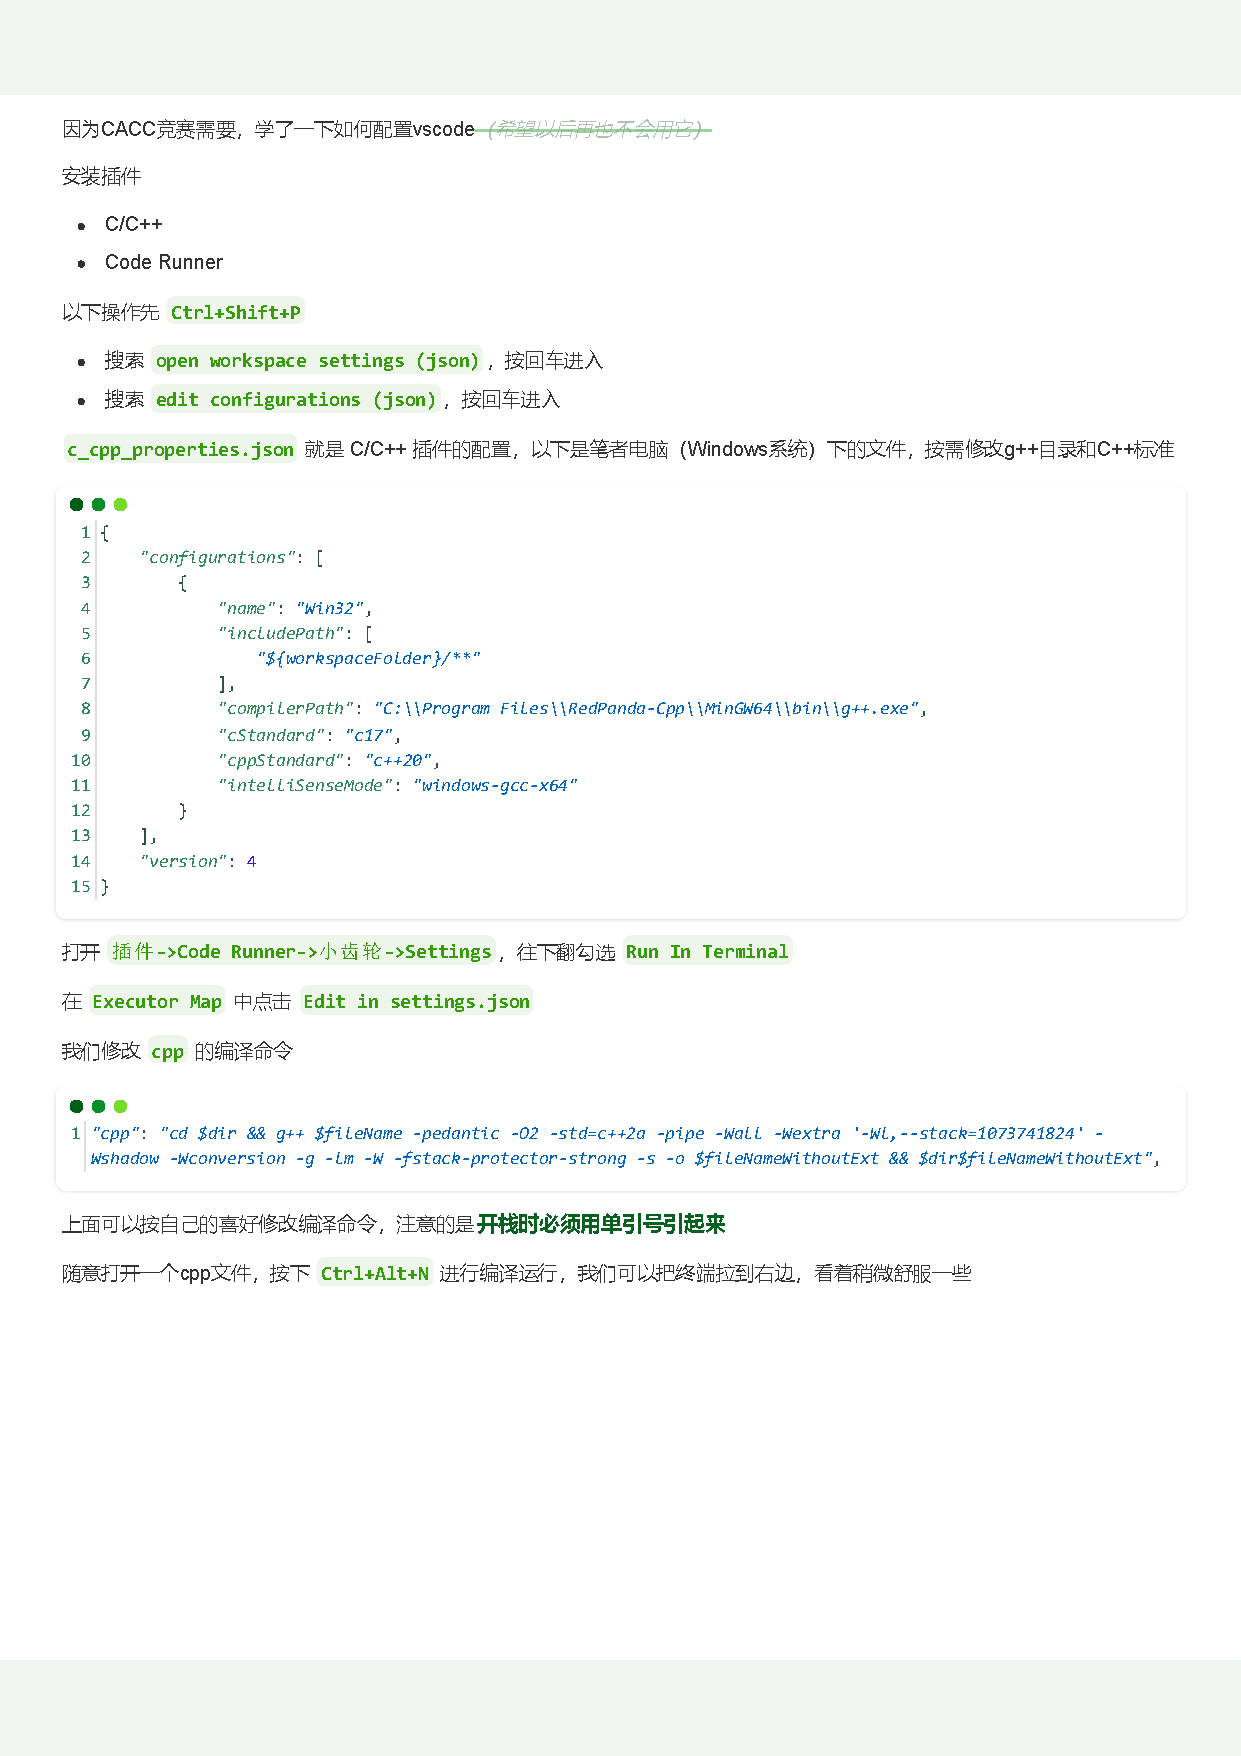
\includepdf[pages=-,scale=0.9]{"../Template/Other/vscode.pdf"}

\newpage

\subsection{数位 dp}

给出一个区间 [l, r], 问有多少数字包含 38 或者 4

\lstinputlisting[style=C++]{"../Template/Other/DP num dp.h"}

\newpage

\subsection{模拟退火}

    \hspace{2em} 用一句话概括过程:如果新状态的解更优则修改答案,否则以一定的概率接收新状态

    \hspace{2em} 定义当前温度为 $T$,新状态 $S'$ 和已知状态 $S$ (新状态由已知状态通过随机的方式得到)之间的能量(值)差为 $\Delta E$ $(\Delta E\ge0)$,则发生状态转移(修改最优解)的概率为

$$
P(\Delta E)=
\begin{cases}
	1 & S'\text{ is better than S}\\
	exp(-\Delta E/T) & \text{otherwise}
\end{cases}
$$

$P.S.$ 

    \hspace{2em} 1. 这里 $E$ 越小代表越接近最优解,实际若 $E$ 越大越接近最优解,可考虑把 $-E$ 作为能量值函数

    \hspace{2em} 2. 为了使得解更为精确,通常不直接取当前解作为答案,而是在退火过程中维护遇到的所有解的最优值

    \hspace{2em} 3. 有时为了使得到的解更有质量,会在模拟退火结束后,以当前温度在得到的解附近多次随机状态,尝试得到更优的解(其过程与模拟退火相似)

    \hspace{2em} 以下代码以\href{https://www.luogu.com.cn/problem/P1337}{P1337 [JSOI2004] 平衡点 / 吊打XXX}(求 $n$ 个点的带权费马点)为例(改了改 wiki 里的代码)

\lstinputlisting[style=C++]{"../Template/Other/Simulated Annealing.h"}

\newpage

\subsection{和哈希}

\textbf{加减,乘除}两对运算中任选一对即可

\textbf{除法慎用,求逆元会使复杂度多一个log}

\lstinputlisting[style=C++]{"../Template/Other/Sum Hash.h"}

\newpage

% \subsection{手写 bitset}
% 
% \textbf{大概是 std::bitset 的 0.87 倍常数}
% 
% \lstinputlisting[style=C++]{"../Template/Other/Bitset.h"}
% 
% \newpage

\subsection{pbds 提供的 umap 代替品}

\begin{lstlisting}[style=C++]
#include<bits/stdc++.h>
#include<ext/pb_ds/assoc_container.hpp>
#include<ext/pb_ds/hash_policy.hpp>
using namespace std;
using namespace __gnu_pbds;
gp_hash_table<pair<int,int>,int> h;
\end{lstlisting}

\subsection{预处理勾股数}

\lstinputlisting[style=C++]{"../Template/Other/PPT.h"}

\subsection{加速 std::bitset 的预处理指令}

\begin{lstlisting}[style=C++]
	#define __AVX__ 1
	#define __AVX2__ 1
	#pragma GCC optimize("Ofast,unroll-loops")
	#pragma GCC target("avx2,bmi,fma,popcnt")
\end{lstlisting}

\subsection{某个交互题 trick}

对于正整数 $x\ (x>1)$,令 $n=x^2$,则 $\lceil \dfrac{n}{1}\rceil,\lceil \dfrac{n}{2}\rceil,\cdots,\lceil \dfrac{n}{x-1}\rceil$ 各不相同 (\href{https://codeforces.com/contest/2135/problem/D2}{CF2135D2})

\newpage

\subsection{一些 Hash class}

\lstinputlisting[style=C++]{"../Template/Other/Hash.h"}

\subsection{质因数个数与因数个数的上界}

\begin{table}[!ht]
	\centering
	\begin{tabular}{|c|c|c|c|c|c|c|c|c|c|}
		\hline
		n$\le$ & $10^{1}$ & $10^{2}$ & $10^{3}$ & $10^{4}$ & $10^{5}$ & $10^{6}$ & $10^{7}$ & $10^{8}$ & $10^{9}$ \\ \hline
		$max\{\omega(n)\}$ & 2 & 3 & 4 & 5 & 6 & 7 & 8 & 8 & 9 \\ \hline
		$max\{d(n)\}$ & 4 & 12 & 32 & 64 & 128 & 240 & 448 & 768 & 1344 \\ \hline
		n$\le$ & $10^{10}$ & $10^{11}$ & $10^{12}$ & $10^{13}$ & $10^{14}$ & $10^{15}$ & $10^{16}$ & $10^{17}$ & $10^{18}$ \\ \hline
		$max\{\omega(n)\}$ & 10 & 10 & 11 & 12 & 12 & 13 & 13 & 14 & 15 \\ \hline
		$max\{d(n)\}$ & 2304 & 4032 & 6720 & 10752 & 17280 & 26880 & 41472 & 64512 & 103680 \\ \hline
	\end{tabular}
\end{table}

\subsection{写在最后(来自 Benq 大神的几句话)}

\begin{lstlisting}[style=C++]
/* stuff you should look for
* int overflow, array bounds
* special cases (n=1?)
* do smth instead of nothing and stay organized
* WRITE STUFF DOWN
* DON'T GET STUCK ON ONE APPROACH
*/
\end{lstlisting}

\end{document}